\chapter{Design and Architecture}
In this chapter an application architecture called Flux will be explained in more detail with examples.  Also it will explain the whole system, the client the server, storage and communication. First the general architecture of client and server as a whole, and then focus on individual parts of the system in more detail, and explain the most interesting parts of the architecture. Reasonin behind some desig choices will albo be included.

\section{Flux}
To explain how Flux application architecture works and behaves, a couple of examples will be presented of differend complexity. Explanation will involve a minimal amount of code, but section \ref{sec:fluximplementation} in chapter \ref{cha:implementation} has more technical information. To get a more general feel of Flux and other architectures revisit section \ref{sec:fluxmvc} in chapter \ref{cha:beckground}.
\subsubsection{The Dispatcher \worry{should be in background}}
The Dispatchers role is to manage all the actions, it doesn't know where the action is going, neither what the payload is. The dispatcher is globally notifying the stores about the actions, and additionaly the stores can be set up to wait for other stores update themselves. With the Dispatcher \emph{waitFor()} method, a \emph{not ready flag} can be set on any particular store that depends on the data from another store. 
\subsection{Simple user action with Flux}\label{sec:simplefluxexample}
The main idea of flux architecture is that it forces one directional dataflow through the system. Any action, be it user action or server action, from the systems perspecive, will originate from the same place, in Flux we call that place the dispatcher. When the focus is scalability, building simple things like triggering a remove operation on a list, may seem cubersome when one needs to follow quite strict rules, such as those proposed in Flux. It might seem that there is a lot of redundand code, but at the end it pays off since it simplifies the impliementation process of other modules when one gets to know the architecture better and have set up all the neccesary nodes. This is very clear by looking at an example below. In Autograder, teachers sometimes have to remove users from a course, or even from the whole system, be it fake users, or dropouts. A list of users is provided for the user:
\begin{figure}[h]
 % \scalebox{1}{% Graphic for TeX using PGF
% Title: /home/tomgli/workspace/github.com/bachopp/thesis/files/chapters/design/graphics/simpleremoveuser.dia
% Creator: Dia v0.97.3
% CreationDate: Fri May  6 18:21:29 2016
% For: tomgli
% \usepackage{tikz}
% The following commands are not supported in PSTricks at present
% We define them conditionally, so when they are implemented,
% this pgf file will use them.
\ifx\du\undefined
  \newlength{\du}
\fi
\setlength{\du}{15\unitlength}
\begin{tikzpicture}
\pgftransformxscale{1.000000}
\pgftransformyscale{-1.000000}
\definecolor{dialinecolor}{rgb}{0.000000, 0.000000, 0.000000}
\pgfsetstrokecolor{dialinecolor}
\definecolor{dialinecolor}{rgb}{1.000000, 1.000000, 1.000000}
\pgfsetfillcolor{dialinecolor}
% image rendering not supported% setfont left to latex
\definecolor{dialinecolor}{rgb}{0.000000, 0.000000, 0.000000}
\pgfsetstrokecolor{dialinecolor}
\node at (48.662500\du,24.782500\du){Triggers action};
\pgfsetlinewidth{0.100000\du}
\pgfsetdash{}{0pt}
\pgfsetdash{}{0pt}
\pgfsetmiterjoin
\pgfsetbuttcap
{
\definecolor{dialinecolor}{rgb}{0.000000, 0.000000, 0.000000}
\pgfsetfillcolor{dialinecolor}
% was here!!!
\pgfsetarrowsend{latex}
\definecolor{dialinecolor}{rgb}{0.000000, 0.000000, 0.000000}
\pgfsetstrokecolor{dialinecolor}
\pgfpathmoveto{\pgfpoint{48.887500\du}{25.062500\du}}
\pgfpathcurveto{\pgfpoint{48.937500\du}{27.862500\du}}{\pgfpoint{51.420701\du}{31.239594\du}}{\pgfpoint{53.268638\du}{31.296658\du}}
\pgfusepath{stroke}
}
% setfont left to latex
\definecolor{dialinecolor}{rgb}{0.000000, 0.000000, 0.000000}
\pgfsetstrokecolor{dialinecolor}
\node[anchor=west] at (35.901642\du,38.651596\du){Store will update and row will not display};
\pgfsetlinewidth{0.100000\du}
\pgfsetdash{}{0pt}
\pgfsetdash{}{0pt}
\pgfsetmiterjoin
\pgfsetbuttcap
{
\definecolor{dialinecolor}{rgb}{0.000000, 0.000000, 0.000000}
\pgfsetfillcolor{dialinecolor}
% was here!!!
\pgfsetarrowsend{latex}
\definecolor{dialinecolor}{rgb}{0.000000, 0.000000, 0.000000}
\pgfsetstrokecolor{dialinecolor}
\pgfpathmoveto{\pgfpoint{35.638700\du}{38.461607\du}}
\pgfpathcurveto{\pgfpoint{34.483865\du}{38.461607\du}}{\pgfpoint{35.490050\du}{32.812892\du}}{\pgfpoint{36.292762\du}{31.683149\du}}
\pgfusepath{stroke}
}
\end{tikzpicture}
}
  \scalebox{1}[1]{{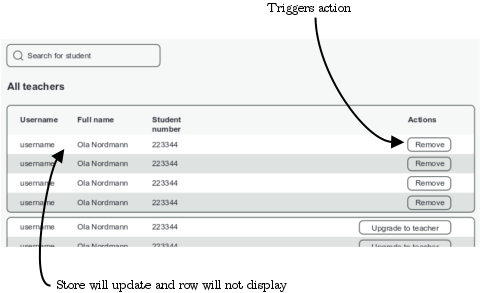
\includegraphics[width=1\linewidth]{graphics/simpleremoveuser.png}}}
  \caption{Representation of course student list view}
  \label{fig:simpleremoveuser}
\end{figure}

User interactions like pressing a button, triggers an action in the system. An action is a method of some \emph{ActionCreators} object. Those ActionCreators are associated with UI elements, they can have a long range of methods in them, depending on how comprehensive the UI elements are and how many interactive elements they have. In this case, example will explain one of the methods - sending an action for removeing the user from course.
\\At any given time the application is in some \emph{state}, one could compare state to the information stored in URL, although state comprises of much more information than URL. The state has the information about who is pressing the button, what course is active etc. More on states in the next section \ref{sec:advancedfluxexample}. State is stored in objects called Stores. When an action to remove a student is being sent, it gets dispatched through a dispatcher (the origin of all changes), and the stores that are interested in this action update themselves according to the information in action payload slightly changing the state of the application.

\begin{figure}[h]
  \scalebox{0.8}{% Graphic for TeX using PGF
% Title: /home/tomgli/workspace/github.com/bachopp/thesis/files/chapters/design/graphics/simplefluxremoveuser.dia
% Creator: Dia v0.97.3
% CreationDate: Mon May  9 16:46:25 2016
% For: tomgli
% \usepackage{tikz}
% The following commands are not supported in PSTricks at present
% We define them conditionally, so when they are implemented,
% this pgf file will use them.
\ifx\du\undefined
  \newlength{\du}
\fi
\setlength{\du}{15\unitlength}
\begin{tikzpicture}
\pgftransformxscale{1.000000}
\pgftransformyscale{-1.000000}
\definecolor{dialinecolor}{rgb}{0.000000, 0.000000, 0.000000}
\pgfsetstrokecolor{dialinecolor}
\definecolor{dialinecolor}{rgb}{1.000000, 1.000000, 1.000000}
\pgfsetfillcolor{dialinecolor}
\definecolor{dialinecolor}{rgb}{1.000000, 1.000000, 1.000000}
\pgfsetfillcolor{dialinecolor}
\fill (28.244400\du,5.226760\du)--(28.244400\du,8.828152\du)--(35.463246\du,8.828152\du)--(35.463246\du,5.226760\du)--cycle;
\pgfsetlinewidth{0.100000\du}
\pgfsetdash{}{0pt}
\pgfsetdash{}{0pt}
\pgfsetmiterjoin
\definecolor{dialinecolor}{rgb}{0.000000, 0.000000, 0.000000}
\pgfsetstrokecolor{dialinecolor}
\draw (28.244400\du,5.226760\du)--(28.244400\du,8.828152\du)--(35.463246\du,8.828152\du)--(35.463246\du,5.226760\du)--cycle;
% setfont left to latex
\definecolor{dialinecolor}{rgb}{0.000000, 0.000000, 0.000000}
\pgfsetstrokecolor{dialinecolor}
\node at (31.853823\du,6.827456\du){View};
% setfont left to latex
\definecolor{dialinecolor}{rgb}{0.000000, 0.000000, 0.000000}
\pgfsetstrokecolor{dialinecolor}
\node at (31.853823\du,7.627456\du){CourseStudentList};
\definecolor{dialinecolor}{rgb}{1.000000, 1.000000, 1.000000}
\pgfsetfillcolor{dialinecolor}
\fill (3.713580\du,5.237260\du)--(3.713580\du,8.838652\du)--(10.103987\du,8.838652\du)--(10.103987\du,5.237260\du)--cycle;
\pgfsetlinewidth{0.100000\du}
\pgfsetdash{}{0pt}
\pgfsetdash{}{0pt}
\pgfsetmiterjoin
\definecolor{dialinecolor}{rgb}{0.000000, 0.000000, 0.000000}
\pgfsetstrokecolor{dialinecolor}
\draw (3.713580\du,5.237260\du)--(3.713580\du,8.838652\du)--(10.103987\du,8.838652\du)--(10.103987\du,5.237260\du)--cycle;
% setfont left to latex
\definecolor{dialinecolor}{rgb}{0.000000, 0.000000, 0.000000}
\pgfsetstrokecolor{dialinecolor}
\node at (6.908784\du,6.837956\du){ActionCreators};
% setfont left to latex
\definecolor{dialinecolor}{rgb}{0.000000, 0.000000, 0.000000}
\pgfsetstrokecolor{dialinecolor}
\node at (6.908784\du,7.637956\du){CourseUsers};
\definecolor{dialinecolor}{rgb}{0.898039, 0.898039, 0.898039}
\pgfsetfillcolor{dialinecolor}
\fill (11.306400\du,5.231230\du)--(11.306400\du,8.832622\du)--(15.403900\du,8.832622\du)--(15.403900\du,5.231230\du)--cycle;
\pgfsetlinewidth{0.100000\du}
\pgfsetdash{}{0pt}
\pgfsetdash{}{0pt}
\pgfsetmiterjoin
\definecolor{dialinecolor}{rgb}{0.000000, 0.000000, 0.000000}
\pgfsetstrokecolor{dialinecolor}
\draw (11.306400\du,5.231230\du)--(11.306400\du,8.832622\du)--(15.403900\du,8.832622\du)--(15.403900\du,5.231230\du)--cycle;
% setfont left to latex
\definecolor{dialinecolor}{rgb}{0.000000, 0.000000, 0.000000}
\pgfsetstrokecolor{dialinecolor}
\node at (13.355150\du,7.231926\du){Dispatcher};
\definecolor{dialinecolor}{rgb}{1.000000, 1.000000, 1.000000}
\pgfsetfillcolor{dialinecolor}
\fill (18.614900\du,5.221790\du)--(18.614900\du,8.823182\du)--(25.313365\du,8.823182\du)--(25.313365\du,5.221790\du)--cycle;
\pgfsetlinewidth{0.100000\du}
\pgfsetdash{}{0pt}
\pgfsetdash{}{0pt}
\pgfsetmiterjoin
\definecolor{dialinecolor}{rgb}{0.000000, 0.000000, 0.000000}
\pgfsetstrokecolor{dialinecolor}
\draw (18.614900\du,5.221790\du)--(18.614900\du,8.823182\du)--(25.313365\du,8.823182\du)--(25.313365\du,5.221790\du)--cycle;
% setfont left to latex
\definecolor{dialinecolor}{rgb}{0.000000, 0.000000, 0.000000}
\pgfsetstrokecolor{dialinecolor}
\node at (21.964132\du,6.822486\du){CourseStudent};
% setfont left to latex
\definecolor{dialinecolor}{rgb}{0.000000, 0.000000, 0.000000}
\pgfsetstrokecolor{dialinecolor}
\node at (21.964132\du,7.622486\du){ListStore};
\pgfsetlinewidth{0.100000\du}
\pgfsetdash{}{0pt}
\pgfsetdash{}{0pt}
\pgfsetbuttcap
{
\definecolor{dialinecolor}{rgb}{0.000000, 0.000000, 0.000000}
\pgfsetfillcolor{dialinecolor}
% was here!!!
\pgfsetarrowsend{latex}
\definecolor{dialinecolor}{rgb}{0.000000, 0.000000, 0.000000}
\pgfsetstrokecolor{dialinecolor}
\draw (10.104000\du,7.037960\du)--(11.306400\du,7.031930\du);
}
\pgfsetlinewidth{0.100000\du}
\pgfsetdash{}{0pt}
\pgfsetdash{}{0pt}
\pgfsetbuttcap
{
\definecolor{dialinecolor}{rgb}{0.000000, 0.000000, 0.000000}
\pgfsetfillcolor{dialinecolor}
% was here!!!
\pgfsetarrowsend{latex}
\definecolor{dialinecolor}{rgb}{0.000000, 0.000000, 0.000000}
\pgfsetstrokecolor{dialinecolor}
\draw (15.403900\du,7.031930\du)--(18.614900\du,7.022486\du);
}
\pgfsetlinewidth{0.100000\du}
\pgfsetdash{}{0pt}
\pgfsetdash{}{0pt}
\pgfsetmiterjoin
\pgfsetbuttcap
{
\definecolor{dialinecolor}{rgb}{0.000000, 0.000000, 0.000000}
\pgfsetfillcolor{dialinecolor}
% was here!!!
\pgfsetarrowsend{latex}
{\pgfsetcornersarced{\pgfpoint{0.000000\du}{0.000000\du}}\definecolor{dialinecolor}{rgb}{0.000000, 0.000000, 0.000000}
\pgfsetstrokecolor{dialinecolor}
\draw (31.853823\du,5.226760\du)--(31.853823\du,4.176760\du)--(6.908784\du,4.176760\du)--(6.908784\du,5.237260\du);
}}
% setfont left to latex
\definecolor{dialinecolor}{rgb}{0.000000, 0.000000, 0.000000}
\pgfsetstrokecolor{dialinecolor}
\node at (19.890111\du,2.751733\du){removeUser()};
% setfont left to latex
\definecolor{dialinecolor}{rgb}{0.000000, 0.000000, 0.000000}
\pgfsetstrokecolor{dialinecolor}
\node at (19.890111\du,3.551733\du){actionType: REMOVE\_USER\_FROM\_COURSE, payload: \{...\}};
% setfont left to latex
\definecolor{dialinecolor}{rgb}{0.000000, 0.000000, 0.000000}
\pgfsetstrokecolor{dialinecolor}
\node at (26.513300\du,6.488150\du){Update};
\pgfsetlinewidth{0.100000\du}
\pgfsetdash{}{0pt}
\pgfsetdash{}{0pt}
\pgfsetbuttcap
{
\definecolor{dialinecolor}{rgb}{0.000000, 0.000000, 0.000000}
\pgfsetfillcolor{dialinecolor}
% was here!!!
\pgfsetarrowsend{latex}
\definecolor{dialinecolor}{rgb}{0.000000, 0.000000, 0.000000}
\pgfsetstrokecolor{dialinecolor}
\draw (25.313365\du,7.022486\du)--(28.244400\du,7.027450\du);
}
% setfont left to latex
\definecolor{dialinecolor}{rgb}{0.000000, 0.000000, 0.000000}
\pgfsetstrokecolor{dialinecolor}
\node at (16.996300\du,6.500290\du){Dispatch};
\definecolor{dialinecolor}{rgb}{1.000000, 1.000000, 1.000000}
\pgfsetfillcolor{dialinecolor}
\pgfpathellipse{\pgfpoint{21.958513\du}{10.950722\du}}{\pgfpoint{3.122513\du}{0\du}}{\pgfpoint{0\du}{1.210632\du}}
\pgfusepath{fill}
\pgfsetlinewidth{0.100000\du}
\pgfsetdash{}{0pt}
\pgfsetdash{}{0pt}
\pgfsetmiterjoin
\definecolor{dialinecolor}{rgb}{0.000000, 0.000000, 0.000000}
\pgfsetstrokecolor{dialinecolor}
\pgfpathellipse{\pgfpoint{21.958513\du}{10.950722\du}}{\pgfpoint{3.122513\du}{0\du}}{\pgfpoint{0\du}{1.210632\du}}
\pgfusepath{stroke}
% setfont left to latex
\definecolor{dialinecolor}{rgb}{0.000000, 0.000000, 0.000000}
\pgfsetstrokecolor{dialinecolor}
\node at (21.958513\du,11.150722\du){update itself};
\pgfsetlinewidth{0.100000\du}
\pgfsetdash{}{0pt}
\pgfsetdash{}{0pt}
\pgfsetbuttcap
{
\definecolor{dialinecolor}{rgb}{0.000000, 0.000000, 0.000000}
\pgfsetfillcolor{dialinecolor}
% was here!!!
\definecolor{dialinecolor}{rgb}{0.000000, 0.000000, 0.000000}
\pgfsetstrokecolor{dialinecolor}
\draw (21.964132\du,8.823182\du)--(21.958500\du,9.740090\du);
}
\end{tikzpicture}
}
  \caption{How removeing user happens with this architecture.}
  \label{fig:simplefluxremoveuser}
\end{figure}

\subsection{Bigger example of user action with Flux}\label{sec:advancedfluxexample}
What makes Flux a great architecture is that more complicated implementations do not differ that much form the simpler ones. The data flow in Flux is one directional, two different views will not communicate directly with eachother, rather they will do so by creating actions, triggering store changes and consequently updating both views. To explain how different views communicate, and how stores and store dependancies work, it is necessay to look at a bigger part of a page not just one single element, and explore the communication between views making up that page.
\\Lets take a look at views responsible for managing groups for courses. There are three main views shown in figure \ref{fig:advancedgroupmanager}, one take care of switching between the courses, one lists available students that have no groups, and group list and manager. Here the top view, switching between courses, is independent of the two below, switching course triggers an API request for new list of students and groups. The buttons for adding students to course communicate with the righ view that lists the group.

\begin{figure}[h]
 % \scalebox{1}{% Graphic for TeX using PGF
% Title: /home/tomgli/workspace/github.com/bachopp/thesis/files/chapters/design/graphics/simpleremoveuser.dia
% Creator: Dia v0.97.3
% CreationDate: Fri May  6 18:21:29 2016
% For: tomgli
% \usepackage{tikz}
% The following commands are not supported in PSTricks at present
% We define them conditionally, so when they are implemented,
% this pgf file will use them.
\ifx\du\undefined
  \newlength{\du}
\fi
\setlength{\du}{15\unitlength}
\begin{tikzpicture}
\pgftransformxscale{1.000000}
\pgftransformyscale{-1.000000}
\definecolor{dialinecolor}{rgb}{0.000000, 0.000000, 0.000000}
\pgfsetstrokecolor{dialinecolor}
\definecolor{dialinecolor}{rgb}{1.000000, 1.000000, 1.000000}
\pgfsetfillcolor{dialinecolor}
% image rendering not supported% setfont left to latex
\definecolor{dialinecolor}{rgb}{0.000000, 0.000000, 0.000000}
\pgfsetstrokecolor{dialinecolor}
\node at (48.662500\du,24.782500\du){Triggers action};
\pgfsetlinewidth{0.100000\du}
\pgfsetdash{}{0pt}
\pgfsetdash{}{0pt}
\pgfsetmiterjoin
\pgfsetbuttcap
{
\definecolor{dialinecolor}{rgb}{0.000000, 0.000000, 0.000000}
\pgfsetfillcolor{dialinecolor}
% was here!!!
\pgfsetarrowsend{latex}
\definecolor{dialinecolor}{rgb}{0.000000, 0.000000, 0.000000}
\pgfsetstrokecolor{dialinecolor}
\pgfpathmoveto{\pgfpoint{48.887500\du}{25.062500\du}}
\pgfpathcurveto{\pgfpoint{48.937500\du}{27.862500\du}}{\pgfpoint{51.420701\du}{31.239594\du}}{\pgfpoint{53.268638\du}{31.296658\du}}
\pgfusepath{stroke}
}
% setfont left to latex
\definecolor{dialinecolor}{rgb}{0.000000, 0.000000, 0.000000}
\pgfsetstrokecolor{dialinecolor}
\node[anchor=west] at (35.901642\du,38.651596\du){Store will update and row will not display};
\pgfsetlinewidth{0.100000\du}
\pgfsetdash{}{0pt}
\pgfsetdash{}{0pt}
\pgfsetmiterjoin
\pgfsetbuttcap
{
\definecolor{dialinecolor}{rgb}{0.000000, 0.000000, 0.000000}
\pgfsetfillcolor{dialinecolor}
% was here!!!
\pgfsetarrowsend{latex}
\definecolor{dialinecolor}{rgb}{0.000000, 0.000000, 0.000000}
\pgfsetstrokecolor{dialinecolor}
\pgfpathmoveto{\pgfpoint{35.638700\du}{38.461607\du}}
\pgfpathcurveto{\pgfpoint{34.483865\du}{38.461607\du}}{\pgfpoint{35.490050\du}{32.812892\du}}{\pgfpoint{36.292762\du}{31.683149\du}}
\pgfusepath{stroke}
}
\end{tikzpicture}
}
  \scalebox{1}[1]{{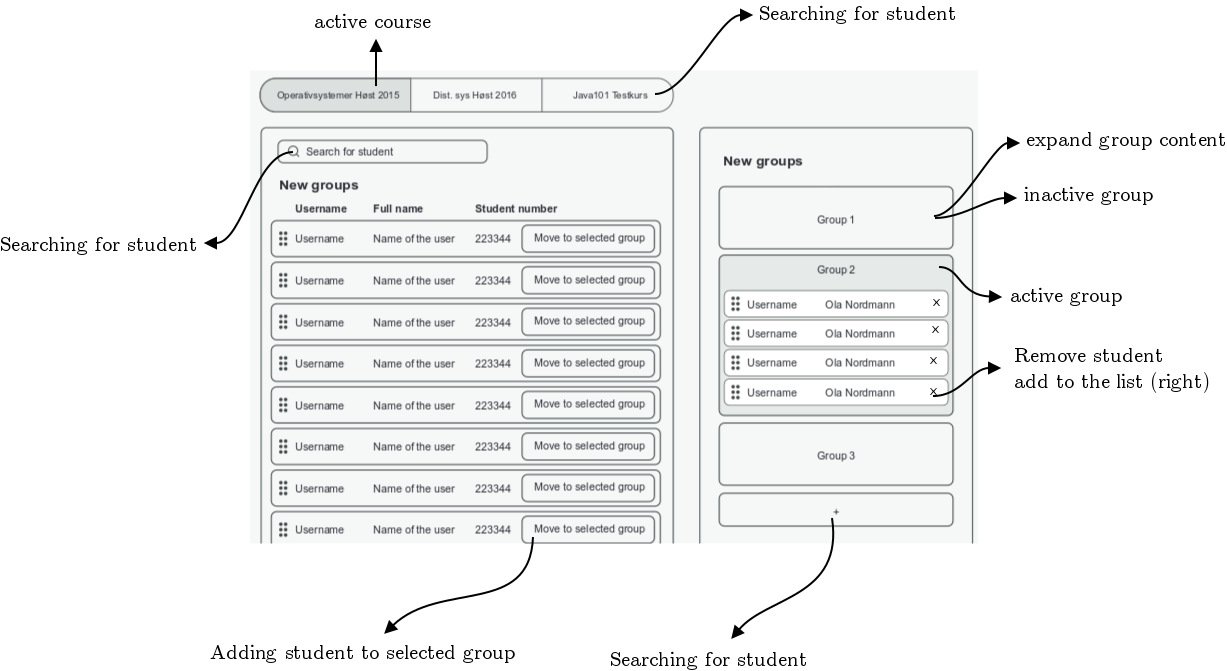
\includegraphics[width=1\linewidth]{graphics/advancedgroupmanager.png}}}
  \caption{Group manager and actions that can be triggered by user}
  \todo{fix figure}
  \label{fig:advancedgroupmanager}
\end{figure}

First a \emph{store} is created, a datastructure that will represent the two views. Lets call it \emph{GroupManagerStore}, this store will have to communicate with another store called \emph{ActiveCourseStore}, that store is responsible for holding data about the current active course in the state. The way this particular example is set up, GroupManagerStore depends on the data in ActiveCourseStore, but at the same time it is impossible for ActiveCourseStore to be ampty while GroupManagerStore requests data from it, because of the way the navigation works in this case. Additionaly a third store is used in the background, since the list of users or students is reused very often while navigating through the course, there is a separate store for student list called \emph{StudentsStore}, other stores that require a list of students will no longer have to request this data from the server, given that another store already requested student lists. For example, both GroupManagerStore and the store from previous example \ref{sec:simplefluxexample} would require a list of students.
\\Given the state shown in figure \ref{fig:advancedgroupmanager}, the user selects a user to be added to the active course, lets go through the flow of data in that case.

\begin{figure}[h]
  \scalebox{0.8}{% Graphic for TeX using PGF
% Title: /home/tomgli/workspace/github.com/bachopp/thesis/files/chapters/design/graphics/advancedfluxaddstudent.dia
% Creator: Dia v0.97.3
% CreationDate: Tue May 10 18:29:14 2016
% For: tomgli
% \usepackage{tikz}
% The following commands are not supported in PSTricks at present
% We define them conditionally, so when they are implemented,
% this pgf file will use them.
\ifx\du\undefined
  \newlength{\du}
\fi
\setlength{\du}{15\unitlength}
\begin{tikzpicture}
\pgftransformxscale{1.000000}
\pgftransformyscale{-1.000000}
\definecolor{dialinecolor}{rgb}{0.000000, 0.000000, 0.000000}
\pgfsetstrokecolor{dialinecolor}
\definecolor{dialinecolor}{rgb}{1.000000, 1.000000, 1.000000}
\pgfsetfillcolor{dialinecolor}
\definecolor{dialinecolor}{rgb}{1.000000, 1.000000, 1.000000}
\pgfsetfillcolor{dialinecolor}
\fill (3.410616\du,5.205062\du)--(3.410616\du,8.806454\du)--(9.000991\du,8.806454\du)--(9.000991\du,5.205062\du)--cycle;
\pgfsetlinewidth{0.100000\du}
\pgfsetdash{}{0pt}
\pgfsetdash{}{0pt}
\pgfsetmiterjoin
\definecolor{dialinecolor}{rgb}{0.000000, 0.000000, 0.000000}
\pgfsetstrokecolor{dialinecolor}
\draw (3.410616\du,5.205062\du)--(3.410616\du,8.806454\du)--(9.000991\du,8.806454\du)--(9.000991\du,5.205062\du)--cycle;
% setfont left to latex
\definecolor{dialinecolor}{rgb}{0.000000, 0.000000, 0.000000}
\pgfsetstrokecolor{dialinecolor}
\node at (6.205804\du,6.805758\du){GroupManager};
% setfont left to latex
\definecolor{dialinecolor}{rgb}{0.000000, 0.000000, 0.000000}
\pgfsetstrokecolor{dialinecolor}
\node at (6.205804\du,7.605758\du){ActionCreators};
\definecolor{dialinecolor}{rgb}{0.945098, 0.945098, 0.945098}
\pgfsetfillcolor{dialinecolor}
\fill (10.661200\du,5.194684\du)--(10.661200\du,8.796076\du)--(15.166074\du,8.796076\du)--(15.166074\du,5.194684\du)--cycle;
\pgfsetlinewidth{0.100000\du}
\pgfsetdash{}{0pt}
\pgfsetdash{}{0pt}
\pgfsetmiterjoin
\definecolor{dialinecolor}{rgb}{0.000000, 0.000000, 0.000000}
\pgfsetstrokecolor{dialinecolor}
\draw (10.661200\du,5.194684\du)--(10.661200\du,8.796076\du)--(15.166074\du,8.796076\du)--(15.166074\du,5.194684\du)--cycle;
% setfont left to latex
\definecolor{dialinecolor}{rgb}{0.000000, 0.000000, 0.000000}
\pgfsetstrokecolor{dialinecolor}
\node[anchor=east] at (14.716074\du,7.195380\du){Dispatcher};
\pgfsetlinewidth{0.100000\du}
\pgfsetdash{}{0pt}
\pgfsetdash{}{0pt}
\pgfsetbuttcap
{
\definecolor{dialinecolor}{rgb}{0.000000, 0.000000, 0.000000}
\pgfsetfillcolor{dialinecolor}
% was here!!!
\pgfsetarrowsend{latex}
\definecolor{dialinecolor}{rgb}{0.000000, 0.000000, 0.000000}
\pgfsetstrokecolor{dialinecolor}
\draw (9.000991\du,7.005758\du)--(10.661200\du,6.995380\du);
}
\pgfsetlinewidth{0.100000\du}
\pgfsetdash{}{0pt}
\pgfsetdash{}{0pt}
\pgfsetmiterjoin
\pgfsetbuttcap
{
\definecolor{dialinecolor}{rgb}{0.000000, 0.000000, 0.000000}
\pgfsetfillcolor{dialinecolor}
% was here!!!
\pgfsetarrowsend{latex}
{\pgfsetcornersarced{\pgfpoint{0.000000\du}{0.000000\du}}\definecolor{dialinecolor}{rgb}{0.000000, 0.000000, 0.000000}
\pgfsetstrokecolor{dialinecolor}
\draw (32.886300\du,4.175120\du)--(32.886300\du,2.204767\du)--(6.205804\du,2.204767\du)--(6.205804\du,5.205062\du);
}}
% setfont left to latex
\definecolor{dialinecolor}{rgb}{0.000000, 0.000000, 0.000000}
\pgfsetstrokecolor{dialinecolor}
\node[anchor=west] at (8.203756\du,0.130673\du){actionType: ADD\_USER\_TO\_GROUP, payload: \{};
% setfont left to latex
\definecolor{dialinecolor}{rgb}{0.000000, 0.000000, 0.000000}
\pgfsetstrokecolor{dialinecolor}
\node[anchor=west] at (8.203756\du,0.930673\du){                                                                      user:\{ name:"test", ... \},};
% setfont left to latex
\definecolor{dialinecolor}{rgb}{0.000000, 0.000000, 0.000000}
\pgfsetstrokecolor{dialinecolor}
\node[anchor=west] at (8.203756\du,1.730673\du){                                                                     \}};
% setfont left to latex
\definecolor{dialinecolor}{rgb}{0.000000, 0.000000, 0.000000}
\pgfsetstrokecolor{dialinecolor}
\node at (28.881375\du,7.103016\du){Update};
% setfont left to latex
\definecolor{dialinecolor}{rgb}{0.000000, 0.000000, 0.000000}
\pgfsetstrokecolor{dialinecolor}
\node at (17.266200\du,6.615950\du){Dispatch};
\definecolor{dialinecolor}{rgb}{1.000000, 1.000000, 1.000000}
\pgfsetfillcolor{dialinecolor}
\fill (30.348400\du,7.095990\du)--(30.348400\du,9.795990\du)--(35.396282\du,9.795990\du)--(35.396282\du,7.095990\du)--cycle;
\pgfsetlinewidth{0.100000\du}
\pgfsetdash{}{0pt}
\pgfsetdash{}{0pt}
\pgfsetmiterjoin
\definecolor{dialinecolor}{rgb}{0.000000, 0.000000, 0.000000}
\pgfsetstrokecolor{dialinecolor}
\draw (30.348400\du,7.095990\du)--(30.348400\du,9.795990\du)--(35.396282\du,9.795990\du)--(35.396282\du,7.095990\du)--cycle;
% setfont left to latex
\definecolor{dialinecolor}{rgb}{0.000000, 0.000000, 0.000000}
\pgfsetstrokecolor{dialinecolor}
\node at (32.872341\du,8.245990\du){View};
% setfont left to latex
\definecolor{dialinecolor}{rgb}{0.000000, 0.000000, 0.000000}
\pgfsetstrokecolor{dialinecolor}
\node at (32.872341\du,9.045990\du){GroupList};
\pgfsetlinewidth{0.100000\du}
\pgfsetdash{}{0pt}
\pgfsetdash{}{0pt}
\pgfsetmiterjoin
\pgfsetbuttcap
{
\definecolor{dialinecolor}{rgb}{0.000000, 0.000000, 0.000000}
\pgfsetfillcolor{dialinecolor}
% was here!!!
\pgfsetarrowsend{latex}
\definecolor{dialinecolor}{rgb}{0.000000, 0.000000, 0.000000}
\pgfsetstrokecolor{dialinecolor}
\pgfpathmoveto{\pgfpoint{26.567545\du}{6.989366\du}}
\pgfpathcurveto{\pgfpoint{27.781345\du}{6.989366\du}}{\pgfpoint{29.148500\du}{5.525120\du}}{\pgfpoint{30.362300\du}{5.525120\du}}
\pgfusepath{stroke}
}
\pgfsetlinewidth{0.100000\du}
\pgfsetdash{}{0pt}
\pgfsetdash{}{0pt}
\pgfsetmiterjoin
\pgfsetbuttcap
{
\definecolor{dialinecolor}{rgb}{0.000000, 0.000000, 0.000000}
\pgfsetfillcolor{dialinecolor}
% was here!!!
\pgfsetarrowsend{latex}
\definecolor{dialinecolor}{rgb}{0.000000, 0.000000, 0.000000}
\pgfsetstrokecolor{dialinecolor}
\pgfpathmoveto{\pgfpoint{26.567545\du}{6.989366\du}}
\pgfpathcurveto{\pgfpoint{27.797545\du}{6.989366\du}}{\pgfpoint{29.118400\du}{8.445990\du}}{\pgfpoint{30.348400\du}{8.445990\du}}
\pgfusepath{stroke}
}
\definecolor{dialinecolor}{rgb}{0.815686, 0.815686, 0.815686}
\pgfsetfillcolor{dialinecolor}
\fill (19.605800\du,8.416370\du)--(19.605800\du,11.230157\du)--(26.299423\du,11.230157\du)--(26.299423\du,8.416370\du)--cycle;
\pgfsetlinewidth{0.100000\du}
\pgfsetdash{}{0pt}
\pgfsetdash{}{0pt}
\pgfsetmiterjoin
\definecolor{dialinecolor}{rgb}{0.000000, 0.000000, 0.000000}
\pgfsetstrokecolor{dialinecolor}
\draw (19.605800\du,8.416370\du)--(19.605800\du,11.230157\du)--(26.299423\du,11.230157\du)--(26.299423\du,8.416370\du)--cycle;
% setfont left to latex
\definecolor{dialinecolor}{rgb}{0.000000, 0.000000, 0.000000}
\pgfsetstrokecolor{dialinecolor}
\node at (22.952612\du,10.023263\du){StudentsStore};
\definecolor{dialinecolor}{rgb}{0.945098, 0.945098, 0.945098}
\pgfsetfillcolor{dialinecolor}
\fill (19.528700\du,2.834900\du)--(19.528700\du,5.648687\du)--(26.231030\du,5.648687\du)--(26.231030\du,2.834900\du)--cycle;
\pgfsetlinewidth{0.100000\du}
\pgfsetdash{}{0pt}
\pgfsetdash{}{0pt}
\pgfsetmiterjoin
\definecolor{dialinecolor}{rgb}{0.000000, 0.000000, 0.000000}
\pgfsetstrokecolor{dialinecolor}
\draw (19.528700\du,2.834900\du)--(19.528700\du,5.648687\du)--(26.231030\du,5.648687\du)--(26.231030\du,2.834900\du)--cycle;
% setfont left to latex
\definecolor{dialinecolor}{rgb}{0.000000, 0.000000, 0.000000}
\pgfsetstrokecolor{dialinecolor}
\node at (22.879865\du,4.441793\du){ActiveCourseStore};
\definecolor{dialinecolor}{rgb}{0.701961, 0.701961, 0.701961}
\pgfsetfillcolor{dialinecolor}
\fill (19.220200\du,5.188670\du)--(19.220200\du,8.790062\du)--(26.567545\du,8.790062\du)--(26.567545\du,5.188670\du)--cycle;
\pgfsetlinewidth{0.100000\du}
\pgfsetdash{}{0pt}
\pgfsetdash{}{0pt}
\pgfsetmiterjoin
\definecolor{dialinecolor}{rgb}{0.000000, 0.000000, 0.000000}
\pgfsetstrokecolor{dialinecolor}
\draw (19.220200\du,5.188670\du)--(19.220200\du,8.790062\du)--(26.567545\du,8.790062\du)--(26.567545\du,5.188670\du)--cycle;
% setfont left to latex
\definecolor{dialinecolor}{rgb}{0.000000, 0.000000, 0.000000}
\pgfsetstrokecolor{dialinecolor}
\node at (22.893873\du,7.189366\du){GroupManagerStore};
\definecolor{dialinecolor}{rgb}{1.000000, 1.000000, 1.000000}
\pgfsetfillcolor{dialinecolor}
\fill (30.362300\du,4.175120\du)--(30.362300\du,6.875120\du)--(35.410182\du,6.875120\du)--(35.410182\du,4.175120\du)--cycle;
\pgfsetlinewidth{0.100000\du}
\pgfsetdash{}{0pt}
\pgfsetdash{}{0pt}
\pgfsetmiterjoin
\definecolor{dialinecolor}{rgb}{0.000000, 0.000000, 0.000000}
\pgfsetstrokecolor{dialinecolor}
\draw (30.362300\du,4.175120\du)--(30.362300\du,6.875120\du)--(35.410182\du,6.875120\du)--(35.410182\du,4.175120\du)--cycle;
% setfont left to latex
\definecolor{dialinecolor}{rgb}{0.000000, 0.000000, 0.000000}
\pgfsetstrokecolor{dialinecolor}
\node at (32.886241\du,5.325120\du){View};
% setfont left to latex
\definecolor{dialinecolor}{rgb}{0.000000, 0.000000, 0.000000}
\pgfsetstrokecolor{dialinecolor}
\node at (32.886241\du,6.125120\du){StudentsList};
% setfont left to latex
\definecolor{dialinecolor}{rgb}{0.000000, 0.000000, 0.000000}
\pgfsetstrokecolor{dialinecolor}
\node[anchor=west] at (15.959804\du,13.559443\du){};
% setfont left to latex
\definecolor{dialinecolor}{rgb}{0.000000, 0.000000, 0.000000}
\pgfsetstrokecolor{dialinecolor}
\node[anchor=west] at (13.227467\du,13.483020\du){students = \ensuremath{[}};
% setfont left to latex
\definecolor{dialinecolor}{rgb}{0.000000, 0.000000, 0.000000}
\pgfsetstrokecolor{dialinecolor}
\node[anchor=west] at (13.227467\du,14.283020\du){\{name:"test",...\}};
% setfont left to latex
\definecolor{dialinecolor}{rgb}{0.000000, 0.000000, 0.000000}
\pgfsetstrokecolor{dialinecolor}
\node[anchor=west] at (13.227467\du,15.083020\du){\{name:"test2,...\}};
% setfont left to latex
\definecolor{dialinecolor}{rgb}{0.000000, 0.000000, 0.000000}
\pgfsetstrokecolor{dialinecolor}
\node[anchor=west] at (13.227467\du,15.883020\du){\{...\}};
% setfont left to latex
\definecolor{dialinecolor}{rgb}{0.000000, 0.000000, 0.000000}
\pgfsetstrokecolor{dialinecolor}
\node[anchor=west] at (13.227467\du,16.683020\du){\ensuremath{]}};
\pgfsetlinewidth{0.100000\du}
\pgfsetdash{}{0pt}
\pgfsetdash{}{0pt}
\pgfsetmiterjoin
\pgfsetbuttcap
{
\definecolor{dialinecolor}{rgb}{0.000000, 0.000000, 0.000000}
\pgfsetfillcolor{dialinecolor}
% was here!!!
\pgfsetarrowsend{latex}
\definecolor{dialinecolor}{rgb}{0.000000, 0.000000, 0.000000}
\pgfsetstrokecolor{dialinecolor}
\pgfpathmoveto{\pgfpoint{19.165519\du}{7.913952\du}}
\pgfpathcurveto{\pgfpoint{16.743793\du}{7.900963\du}}{\pgfpoint{16.197224\du}{9.199064\du}}{\pgfpoint{16.213049\du}{12.771493\du}}
\pgfusepath{stroke}
}
% setfont left to latex
\definecolor{dialinecolor}{rgb}{0.000000, 0.000000, 0.000000}
\pgfsetstrokecolor{dialinecolor}
\node at (14.768438\du,11.523947\du){before};
\pgfsetlinewidth{0.100000\du}
\pgfsetdash{}{0pt}
\pgfsetdash{}{0pt}
\pgfsetbuttcap
{
\definecolor{dialinecolor}{rgb}{0.000000, 0.000000, 0.000000}
\pgfsetfillcolor{dialinecolor}
% was here!!!
\pgfsetarrowsend{latex}
\definecolor{dialinecolor}{rgb}{0.000000, 0.000000, 0.000000}
\pgfsetstrokecolor{dialinecolor}
\draw (19.493473\du,14.990278\du)--(22.539314\du,14.990278\du);
}
% setfont left to latex
\definecolor{dialinecolor}{rgb}{0.000000, 0.000000, 0.000000}
\pgfsetstrokecolor{dialinecolor}
\node at (20.654060\du,14.674666\du){update};
% setfont left to latex
\definecolor{dialinecolor}{rgb}{0.000000, 0.000000, 0.000000}
\pgfsetstrokecolor{dialinecolor}
\node[anchor=west] at (23.334563\du,13.481594\du){students = \ensuremath{[}};
% setfont left to latex
\definecolor{dialinecolor}{rgb}{0.000000, 0.000000, 0.000000}
\pgfsetstrokecolor{dialinecolor}
\node[anchor=west] at (23.334563\du,14.281594\du){\{name:"test",...\}};
% setfont left to latex
\definecolor{dialinecolor}{rgb}{0.000000, 0.000000, 0.000000}
\pgfsetstrokecolor{dialinecolor}
\node[anchor=west] at (23.334563\du,15.081594\du){\{name:"test2,...\}};
% setfont left to latex
\definecolor{dialinecolor}{rgb}{0.000000, 0.000000, 0.000000}
\pgfsetstrokecolor{dialinecolor}
\node[anchor=west] at (23.334563\du,15.881594\du){\{...\}};
% setfont left to latex
\definecolor{dialinecolor}{rgb}{0.000000, 0.000000, 0.000000}
\pgfsetstrokecolor{dialinecolor}
\node[anchor=west] at (23.334563\du,16.681594\du){\ensuremath{]}};
\pgfsetlinewidth{0.100000\du}
\pgfsetdash{}{0pt}
\pgfsetdash{}{0pt}
\pgfsetbuttcap
{
\definecolor{dialinecolor}{rgb}{0.000000, 0.000000, 0.000000}
\pgfsetfillcolor{dialinecolor}
% was here!!!
\definecolor{dialinecolor}{rgb}{0.000000, 0.000000, 0.000000}
\pgfsetstrokecolor{dialinecolor}
\draw (23.652346\du,14.293351\du)--(29.397033\du,14.293351\du);
}
\pgfsetlinewidth{0.100000\du}
\pgfsetdash{}{0pt}
\pgfsetdash{}{0pt}
\pgfsetbuttcap
{
\definecolor{dialinecolor}{rgb}{0.000000, 0.000000, 0.000000}
\pgfsetfillcolor{dialinecolor}
% was here!!!
\pgfsetarrowsend{latex}
\definecolor{dialinecolor}{rgb}{0.000000, 0.000000, 0.000000}
\pgfsetstrokecolor{dialinecolor}
\draw (15.166074\du,6.995380\du)--(19.220200\du,6.989366\du);
}
\pgfsetlinewidth{0.100000\du}
\pgfsetdash{{\pgflinewidth}{0.200000\du}}{0cm}
\pgfsetdash{{\pgflinewidth}{0.200000\du}}{0cm}
\pgfsetmiterjoin
\definecolor{dialinecolor}{rgb}{0.000000, 0.000000, 0.000000}
\pgfsetstrokecolor{dialinecolor}
\pgfpathellipse{\pgfpoint{28.664294\du}{7.015184\du}}{\pgfpoint{2.479850\du}{0\du}}{\pgfpoint{0\du}{2.330956\du}}
\pgfusepath{stroke}
% setfont left to latex
\definecolor{dialinecolor}{rgb}{0.000000, 0.000000, 0.000000}
\pgfsetstrokecolor{dialinecolor}
\node at (28.664294\du,7.210184\du){};
\pgfsetlinewidth{0.100000\du}
\pgfsetdash{}{0pt}
\pgfsetdash{}{0pt}
\pgfsetmiterjoin
\pgfsetbuttcap
{
\definecolor{dialinecolor}{rgb}{0.000000, 0.000000, 0.000000}
\pgfsetfillcolor{dialinecolor}
% was here!!!
\pgfsetarrowsstart{latex}
\definecolor{dialinecolor}{rgb}{0.000000, 0.000000, 0.000000}
\pgfsetstrokecolor{dialinecolor}
\pgfpathmoveto{\pgfpoint{28.735545\du}{9.416979\du}}
\pgfpathcurveto{\pgfpoint{28.735220\du}{11.175743\du}}{\pgfpoint{29.380741\du}{11.769586\du}}{\pgfpoint{30.077157\du}{11.769586\du}}
\pgfusepath{stroke}
}
% setfont left to latex
\definecolor{dialinecolor}{rgb}{0.000000, 0.000000, 0.000000}
\pgfsetstrokecolor{dialinecolor}
\node[anchor=west] at (30.253933\du,11.999395\du){EventEmitter};
\end{tikzpicture}
}
  \caption{How removeing user happens with this architecture.}
  \label{fig:advancedfluxaddstudent}
\end{figure}

When the user presses the button, one of \emph{GroupManagerActionCreators} method is called, this dispatches the action via the Dispatcher. GroupManagerStore is dependant on the data from StudentsStore, but in current state StudentsStore is not empty so it returns immidietly \todo{write about how data is stored in stores, about utils etc.}

\section{Web app}
Architecture of the Autograder system describes the high level structures developed while working on the application. Choice of software architecture, software models on both front and back-end are crucial aspects of creating good application.
\subsection{Software architecture}
Autograder is an application for teachers and students, the new version is going to be running on local university network and is going to be accessible from anywhere on the internet. Primary use for teachers is new creating courses in the system, that are associated with the courses at the university, each course has a GitHub repository associated with it, and configured to the needs of that course. This means that an implementation of GitHub integration needs to be created, this is mainly the focus of back-end part of the software, still the front-end, or web client, needs to be designed in such a way to enable the
 use of such integration. The client is not supposed to serve as an alternative view of GitHub repositories, GitHub is mainly used as a place to easily store source code, and its login authentication API. The client needs to be able to display courses that a student is enrolled into, assignments that the teacher has published to that course, that also involves group assignments.
\\Although the data is stored in the database, manipulation of that data is done on the client side, and then sent further to the back-end for interpretation and updating the storage. Similarly it is also possible to update the client from the back-end, either directly or through the actions of another client. The user interface updates in real time, as an example, lets take a teacher that is assigning students to group assignments, teacher is using an interactive interface to manipulate the users into selected groups, the student is simultaneously notified in real time when he gets assigned to a new group without the need of refreshing the page, similar things would be new teachers in course, requests for teacher upgrade, deadline and slipdays updates. Teachers can be notified when a new student has enrolled to course, or one of the students has exceeded his slip-days for an assignment. Real time updates are possible due to the connection protocol used in the application. When a client connects to the Autograder server, client application requests for a protocol upgrade, from then on all data transfer is done through \emph{websocket protocol}\cite{websocket}. This enables the server to push its updates to all clients, without being explicitly asked about it by them.
\\The reasoning behind real-time update system was that notifications and responsiveness of user interface was one of the primary reasons for developing this solution. Although one could argue that order methods of updating the UI and notifications would be sufficient, like polling or long-polling - that is frequent client requests for update from the server, websocket protocol has no obvious disadvantages to the presented solution, and at the same time opens possibilities for further upgrades of the system, like chat functionality, which could be utilized for questions related to assignments.
\subsection{Front-end}
Front-end web applications are written in JavaScript, or at least have to be transpiled to JavaScript for the browsers to be able to understand it. Applications in JS, are single threaded...
\todo{single threaded approach}

\section{Server}
Back-end solution is not the main focus of this application. Nonetheless a working temporary server needed to be put together, as well as database to store mock data and to test the logical functionality of the system on the front-end and the way the data is being communicated between the two ends.
\subsection{Server}
The server is written in Go, for this purpose there was no real  preference as to what language to use, but assumptions were made that the final server will also be written in Go, therefore it was an obvious choice. Client is designed with WebSocket in mind, the simplest way to implement that on server side is to use Gorilla websocket Go package that can handle WebSocket messages. This was implemented with almost no effort, but the next step is to create logic for handling all the different requests that come from the client. For this purpose, when a server receives a message through WebSocket, a new \emph{goroutine} is fired out, since they are very lightweigh a lot of requests can be potentially handled at the same time. Every requests goes through a simple multiplexer that figures out, based on the message header, what kind of request is made, then it uses the payload to retrieve specific data. As and exaple let's take a user that requested to see all its courses by going to the course overview page, that lists courses that the user is associated with.

\begin{figure}[h]
  % Graphic for TeX using PGF
% Title: /home/tomgli/workspace/github.com/bachopp/thesis/files/chapters/design/graphs/serverwebsocket.dia
% Creator: Dia v0.97.3
% CreationDate: Sat Apr 23 14:55:21 2016
% For: tomgli
% \usepackage{tikz}
% The following commands are not supported in PSTricks at present
% We define them conditionally, so when they are implemented,
% this pgf file will use them.
\ifx\du\undefined
  \newlength{\du}
\fi
\setlength{\du}{15\unitlength}
\begin{tikzpicture}
\pgftransformxscale{1.000000}
\pgftransformyscale{-1.000000}
\definecolor{dialinecolor}{rgb}{0.000000, 0.000000, 0.000000}
\pgfsetstrokecolor{dialinecolor}
\definecolor{dialinecolor}{rgb}{1.000000, 1.000000, 1.000000}
\pgfsetfillcolor{dialinecolor}
\definecolor{dialinecolor}{rgb}{1.000000, 1.000000, 1.000000}
\pgfsetfillcolor{dialinecolor}
\fill (16.302398\du,9.285788\du)--(16.302398\du,11.185788\du)--(22.509898\du,11.185788\du)--(22.509898\du,9.285788\du)--cycle;
\pgfsetlinewidth{0.100000\du}
\pgfsetdash{}{0pt}
\pgfsetdash{}{0pt}
\pgfsetmiterjoin
\definecolor{dialinecolor}{rgb}{0.000000, 0.000000, 0.000000}
\pgfsetstrokecolor{dialinecolor}
\draw (16.302398\du,9.285788\du)--(16.302398\du,11.185788\du)--(22.509898\du,11.185788\du)--(22.509898\du,9.285788\du)--cycle;
% setfont left to latex
\definecolor{dialinecolor}{rgb}{0.000000, 0.000000, 0.000000}
\pgfsetstrokecolor{dialinecolor}
\node at (19.406148\du,10.435788\du){request courses};
\definecolor{dialinecolor}{rgb}{1.000000, 1.000000, 1.000000}
\pgfsetfillcolor{dialinecolor}
\fill (20.877987\du,6.200760\du)--(20.877987\du,8.100760\du)--(27.085487\du,8.100760\du)--(27.085487\du,6.200760\du)--cycle;
\pgfsetlinewidth{0.100000\du}
\pgfsetdash{}{0pt}
\pgfsetdash{}{0pt}
\pgfsetmiterjoin
\definecolor{dialinecolor}{rgb}{0.000000, 0.000000, 0.000000}
\pgfsetstrokecolor{dialinecolor}
\draw (20.877987\du,6.200760\du)--(20.877987\du,8.100760\du)--(27.085487\du,8.100760\du)--(27.085487\du,6.200760\du)--cycle;
% setfont left to latex
\definecolor{dialinecolor}{rgb}{0.000000, 0.000000, 0.000000}
\pgfsetstrokecolor{dialinecolor}
\node at (23.981737\du,7.350760\du){websocket};
\definecolor{dialinecolor}{rgb}{1.000000, 1.000000, 1.000000}
\pgfsetfillcolor{dialinecolor}
\fill (29.928944\du,6.207449\du)--(29.928944\du,8.107449\du)--(36.136444\du,8.107449\du)--(36.136444\du,6.207449\du)--cycle;
\pgfsetlinewidth{0.100000\du}
\pgfsetdash{}{0pt}
\pgfsetdash{}{0pt}
\pgfsetmiterjoin
\definecolor{dialinecolor}{rgb}{0.000000, 0.000000, 0.000000}
\pgfsetstrokecolor{dialinecolor}
\draw (29.928944\du,6.207449\du)--(29.928944\du,8.107449\du)--(36.136444\du,8.107449\du)--(36.136444\du,6.207449\du)--cycle;
% setfont left to latex
\definecolor{dialinecolor}{rgb}{0.000000, 0.000000, 0.000000}
\pgfsetstrokecolor{dialinecolor}
\node at (33.032694\du,7.357449\du){websocket};
\pgfsetlinewidth{0.100000\du}
\pgfsetdash{}{0pt}
\pgfsetdash{}{0pt}
\pgfsetbuttcap
{
\definecolor{dialinecolor}{rgb}{0.000000, 0.000000, 0.000000}
\pgfsetfillcolor{dialinecolor}
% was here!!!
\pgfsetarrowsstart{stealth}
\pgfsetarrowsend{latex}
\definecolor{dialinecolor}{rgb}{0.000000, 0.000000, 0.000000}
\pgfsetstrokecolor{dialinecolor}
\draw (27.085487\du,7.150760\du)--(29.928944\du,7.157449\du);
}
\pgfsetlinewidth{0.100000\du}
\pgfsetdash{}{0pt}
\pgfsetdash{}{0pt}
\pgfsetmiterjoin
\pgfsetbuttcap
{
\definecolor{dialinecolor}{rgb}{0.000000, 0.000000, 0.000000}
\pgfsetfillcolor{dialinecolor}
% was here!!!
\pgfsetarrowsstart{latex}
\pgfsetarrowsend{latex}
{\pgfsetcornersarced{\pgfpoint{0.000000\du}{0.000000\du}}\definecolor{dialinecolor}{rgb}{0.000000, 0.000000, 0.000000}
\pgfsetstrokecolor{dialinecolor}
\draw (19.406148\du,9.285788\du)--(19.406148\du,7.150760\du)--(20.877987\du,7.150760\du);
}}
\definecolor{dialinecolor}{rgb}{1.000000, 1.000000, 1.000000}
\pgfsetfillcolor{dialinecolor}
\fill (34.454423\du,9.594869\du)--(34.454423\du,11.494869\du)--(40.661923\du,11.494869\du)--(40.661923\du,9.594869\du)--cycle;
\pgfsetlinewidth{0.100000\du}
\pgfsetdash{}{0pt}
\pgfsetdash{}{0pt}
\pgfsetmiterjoin
\definecolor{dialinecolor}{rgb}{0.000000, 0.000000, 0.000000}
\pgfsetstrokecolor{dialinecolor}
\draw (34.454423\du,9.594869\du)--(34.454423\du,11.494869\du)--(40.661923\du,11.494869\du)--(40.661923\du,9.594869\du)--cycle;
% setfont left to latex
\definecolor{dialinecolor}{rgb}{0.000000, 0.000000, 0.000000}
\pgfsetstrokecolor{dialinecolor}
\node at (37.558173\du,10.744869\du){mux};
\pgfsetlinewidth{0.100000\du}
\pgfsetdash{}{0pt}
\pgfsetdash{}{0pt}
\pgfsetmiterjoin
\pgfsetbuttcap
{
\definecolor{dialinecolor}{rgb}{0.000000, 0.000000, 0.000000}
\pgfsetfillcolor{dialinecolor}
% was here!!!
\pgfsetarrowsstart{stealth}
\pgfsetarrowsend{latex}
{\pgfsetcornersarced{\pgfpoint{0.000000\du}{0.000000\du}}\definecolor{dialinecolor}{rgb}{0.000000, 0.000000, 0.000000}
\pgfsetstrokecolor{dialinecolor}
\draw (36.136444\du,7.157449\du)--(37.558173\du,7.157449\du)--(37.558173\du,9.594869\du);
}}
\definecolor{dialinecolor}{rgb}{1.000000, 1.000000, 1.000000}
\pgfsetfillcolor{dialinecolor}
\fill (34.525134\du,13.625374\du)--(34.525134\du,15.525374\du)--(40.732634\du,15.525374\du)--(40.732634\du,13.625374\du)--cycle;
\pgfsetlinewidth{0.100000\du}
\pgfsetdash{}{0pt}
\pgfsetdash{}{0pt}
\pgfsetmiterjoin
\definecolor{dialinecolor}{rgb}{0.000000, 0.000000, 0.000000}
\pgfsetstrokecolor{dialinecolor}
\draw (34.525134\du,13.625374\du)--(34.525134\du,15.525374\du)--(40.732634\du,15.525374\du)--(40.732634\du,13.625374\du)--cycle;
% setfont left to latex
\definecolor{dialinecolor}{rgb}{0.000000, 0.000000, 0.000000}
\pgfsetstrokecolor{dialinecolor}
\node at (37.628884\du,14.775374\du){ retrieve data};
\pgfsetlinewidth{0.100000\du}
\pgfsetdash{}{0pt}
\pgfsetdash{}{0pt}
\pgfsetbuttcap
\pgfsetmiterjoin
\pgfsetlinewidth{0.100000\du}
\pgfsetbuttcap
\pgfsetmiterjoin
\pgfsetdash{}{0pt}
\definecolor{dialinecolor}{rgb}{1.000000, 1.000000, 1.000000}
\pgfsetfillcolor{dialinecolor}
\pgfpathmoveto{\pgfpoint{36.459331\du}{17.943065\du}}
\pgfpathcurveto{\pgfpoint{36.926021\du}{17.668065\du}}{\pgfpoint{37.159366\du}{17.576398\du}}{\pgfpoint{37.626056\du}{17.576398\du}}
\pgfpathcurveto{\pgfpoint{38.092746\du}{17.576398\du}}{\pgfpoint{38.326091\du}{17.668065\du}}{\pgfpoint{38.792781\du}{17.943065\du}}
\pgfpathlineto{\pgfpoint{38.792781\du}{19.409731\du}}
\pgfpathcurveto{\pgfpoint{38.326091\du}{19.684731\du}}{\pgfpoint{38.092746\du}{19.776398\du}}{\pgfpoint{37.626056\du}{19.776398\du}}
\pgfpathcurveto{\pgfpoint{37.159366\du}{19.776398\du}}{\pgfpoint{36.926021\du}{19.684731\du}}{\pgfpoint{36.459331\du}{19.409731\du}}
\pgfpathlineto{\pgfpoint{36.459331\du}{17.943065\du}}
\pgfusepath{fill}
\definecolor{dialinecolor}{rgb}{0.000000, 0.000000, 0.000000}
\pgfsetstrokecolor{dialinecolor}
\pgfpathmoveto{\pgfpoint{36.459331\du}{17.943065\du}}
\pgfpathcurveto{\pgfpoint{36.926021\du}{17.668065\du}}{\pgfpoint{37.159366\du}{17.576398\du}}{\pgfpoint{37.626056\du}{17.576398\du}}
\pgfpathcurveto{\pgfpoint{38.092746\du}{17.576398\du}}{\pgfpoint{38.326091\du}{17.668065\du}}{\pgfpoint{38.792781\du}{17.943065\du}}
\pgfpathlineto{\pgfpoint{38.792781\du}{19.409731\du}}
\pgfpathcurveto{\pgfpoint{38.326091\du}{19.684731\du}}{\pgfpoint{38.092746\du}{19.776398\du}}{\pgfpoint{37.626056\du}{19.776398\du}}
\pgfpathcurveto{\pgfpoint{37.159366\du}{19.776398\du}}{\pgfpoint{36.926021\du}{19.684731\du}}{\pgfpoint{36.459331\du}{19.409731\du}}
\pgfpathlineto{\pgfpoint{36.459331\du}{17.943065\du}}
\pgfusepath{stroke}
\pgfsetbuttcap
\pgfsetmiterjoin
\pgfsetdash{}{0pt}
\definecolor{dialinecolor}{rgb}{0.000000, 0.000000, 0.000000}
\pgfsetstrokecolor{dialinecolor}
\pgfpathmoveto{\pgfpoint{36.459331\du}{17.943065\du}}
\pgfpathcurveto{\pgfpoint{36.926021\du}{18.218065\du}}{\pgfpoint{37.159366\du}{18.309731\du}}{\pgfpoint{37.626056\du}{18.309731\du}}
\pgfpathcurveto{\pgfpoint{38.092746\du}{18.309731\du}}{\pgfpoint{38.326091\du}{18.218065\du}}{\pgfpoint{38.792781\du}{17.943065\du}}
\pgfusepath{stroke}
% setfont left to latex
\definecolor{dialinecolor}{rgb}{0.000000, 0.000000, 0.000000}
\pgfsetstrokecolor{dialinecolor}
\node at (37.626056\du,19.059731\du){DB};
\pgfsetlinewidth{0.100000\du}
\pgfsetdash{}{0pt}
\pgfsetdash{}{0pt}
\pgfsetbuttcap
{
\definecolor{dialinecolor}{rgb}{0.000000, 0.000000, 0.000000}
\pgfsetfillcolor{dialinecolor}
% was here!!!
\pgfsetarrowsstart{stealth}
\pgfsetarrowsend{latex}
\definecolor{dialinecolor}{rgb}{0.000000, 0.000000, 0.000000}
\pgfsetstrokecolor{dialinecolor}
\draw (37.628884\du,15.525374\du)--(37.627087\du,17.527982\du);
}
% setfont left to latex
\definecolor{dialinecolor}{rgb}{0.000000, 0.000000, 0.000000}
\pgfsetstrokecolor{dialinecolor}
\node[anchor=west] at (27.417906\du,6.290138\du){API};
% setfont left to latex
\definecolor{dialinecolor}{rgb}{0.000000, 0.000000, 0.000000}
\pgfsetstrokecolor{dialinecolor}
\node[anchor=west] at (37.851566\du,8.215510\du){ActionType};
% setfont left to latex
\definecolor{dialinecolor}{rgb}{0.000000, 0.000000, 0.000000}
\pgfsetstrokecolor{dialinecolor}
\node[anchor=west] at (30.110587\du,12.493653\du){Payload};
\pgfsetlinewidth{0.100000\du}
\pgfsetdash{}{0pt}
\pgfsetdash{}{0pt}
\pgfsetmiterjoin
\pgfsetbuttcap
{
\definecolor{dialinecolor}{rgb}{0.000000, 0.000000, 0.000000}
\pgfsetfillcolor{dialinecolor}
% was here!!!
\pgfsetarrowsstart{stealth}
{\pgfsetcornersarced{\pgfpoint{0.000000\du}{0.000000\du}}\definecolor{dialinecolor}{rgb}{0.000000, 0.000000, 0.000000}
\pgfsetstrokecolor{dialinecolor}
\draw (40.661923\du,10.544869\du)--(41.782634\du,10.544869\du)--(41.782634\du,14.575374\du)--(40.732634\du,14.575374\du);
}}
\pgfsetlinewidth{0.100000\du}
\pgfsetdash{}{0pt}
\pgfsetdash{}{0pt}
\pgfsetmiterjoin
\pgfsetbuttcap
{
\definecolor{dialinecolor}{rgb}{0.000000, 0.000000, 0.000000}
\pgfsetfillcolor{dialinecolor}
% was here!!!
\pgfsetarrowsend{latex}
{\pgfsetcornersarced{\pgfpoint{0.000000\du}{0.000000\du}}\definecolor{dialinecolor}{rgb}{0.000000, 0.000000, 0.000000}
\pgfsetstrokecolor{dialinecolor}
\draw (34.454423\du,10.544869\du)--(33.404423\du,10.544869\du)--(33.404423\du,14.575374\du)--(34.525134\du,14.575374\du);
}}
% setfont left to latex
\definecolor{dialinecolor}{rgb}{0.000000, 0.000000, 0.000000}
\pgfsetstrokecolor{dialinecolor}
\node[anchor=west] at (41.973455\du,12.547141\du){Data};
% setfont left to latex
\definecolor{dialinecolor}{rgb}{0.000000, 0.000000, 0.000000}
\pgfsetstrokecolor{dialinecolor}
\node[anchor=west] at (34.341777\du,4.576531\du){Server};
% setfont left to latex
\definecolor{dialinecolor}{rgb}{0.000000, 0.000000, 0.000000}
\pgfsetstrokecolor{dialinecolor}
\node[anchor=west] at (21.487464\du,4.641961\du){Client};
\pgfsetlinewidth{0.100000\du}
\pgfsetdash{{\pgflinewidth}{0.200000\du}}{0cm}
\pgfsetdash{{\pgflinewidth}{0.200000\du}}{0cm}
\pgfsetbuttcap
{
\definecolor{dialinecolor}{rgb}{0.549020, 0.549020, 0.549020}
\pgfsetfillcolor{dialinecolor}
% was here!!!
\definecolor{dialinecolor}{rgb}{0.549020, 0.549020, 0.549020}
\pgfsetstrokecolor{dialinecolor}
\draw (28.425794\du,1.681021\du)--(28.425794\du,20.764836\du);
}
\pgfsetlinewidth{0.100000\du}
\pgfsetdash{{\pgflinewidth}{0.200000\du}}{0cm}
\pgfsetdash{{\pgflinewidth}{0.200000\du}}{0cm}
\pgfsetbuttcap
{
\definecolor{dialinecolor}{rgb}{0.000000, 0.000000, 0.000000}
\pgfsetfillcolor{dialinecolor}
% was here!!!
\definecolor{dialinecolor}{rgb}{0.000000, 0.000000, 0.000000}
\pgfsetstrokecolor{dialinecolor}
\draw (19.406148\du,11.185788\du)--(19.408610\du,12.750667\du);
}
\end{tikzpicture}

  \caption{How requests are handled on the server}
  \label{fig:serverwebsocket}
\end{figure}

The server is also serving three static files, main.js, index.html, and style.css. These are retrieved by the client with the initial GET request, from then on server is not receivein any new GET requests but rather communicates through websocket. This is a bit different than traditionall communication with GET and POST. Also when the client goes directly to a specific URL like "http://www.autograder.no/teacher/results/dat100" server should respond only with the static data and not care about the path after the domainname / IP, since this part is taken care of by the client side routing, as explained in section \ref{sec:softwaresolution}. Further, when a user navigates through the application no GET requests are being made.
\\ActionType that the multiplexer pivots at, is a string representing something similar to what a REST API would typically use. ActionType is a string describing an event, and Payload is the data that is needed to make the changes. Typical HTML form send through websocket, would look like that:
\todo{use form from course settings here}
latex online collaboration\lstinputlisting[label=lst:websocketapi]{listings/websocketapi.js}

This means in short that the client requests roles for username "tokams", server should respond with the same actionType, and as a payload insert relevant data.

\subsection {Database}
Database is running on mysql-server, it's separate from the main go server, it communicates with the server with the help of go sql/package and a 3rd party mysql driver \cite{ziutek}. It is a relational database, that represents the data of users and courses. Although not necessary, it was helpfoul to implement test database solution, to explore the possibilities for back end, and se front to back flow of the data. Database was designed with standard ER diagrams first, and then set up on local machines.
It is discuissed in a bit more technical way in section \ref{sec:database}, and the figure \ref{fig:databaseer}.

